\documentclass{standalone}
\usepackage{pgfplots}
\usetikzlibrary{intersections}
\usepgfplotslibrary{fillbetween}
\pgfplotsset{compat=1.7}

\begin{document}
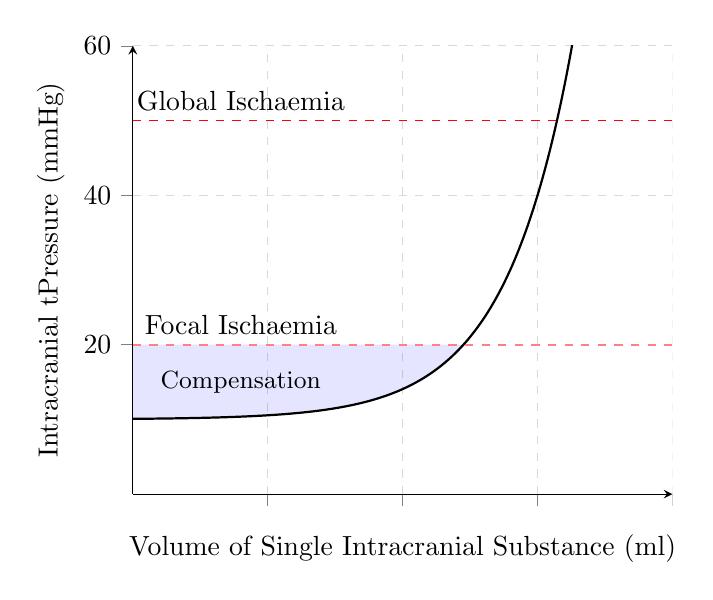
\begin{tikzpicture}


\begin{axis}[
        axis lines=middle,
        grid = major,
        grid style={dashed, gray!30},
	ymin = 0,
	ymax = 60,
	xmin = 0,
	xmax =40,
	xticklabels={},
	 ylabel near ticks,
	xlabel near ticks,
        xlabel=Volume of Single Intracranial Substance (ml),
        ylabel=Intracranial tPressure (mmHg),
        tick align=outside,
        enlargelimits=false]

\addplot[name path =curve, domain=0:24.5, black, thick,samples=500] {10+30*e^(0.2*(x-30))};
\addplot[domain=24.5:40, black, thick,samples=500] {10+30*e^(0.2*(x-30))};


\addplot[domain=0:40, red,dashed,thin]{50} node[above, black,pos=0.2]{Global Ischaemia};
\addplot[domain=0:40, red!50,dashed,thick]{20} node[above, black, pos=0.2]{Focal Ischaemia};

\plot[name path=focal, domain=0:24.5, draw=none] {20};	
\addplot[fill=blue,opacity=0.1] fill between [of=curve and focal];

\node[black, font=\small] at (axis cs: 8,15) {Compensation};

\end{axis}

\end{tikzpicture} 
\end{document}